This test uses $F$ in equation~\eqref{eq:gen-smear} as a simple sum of similar loops,
specifically plaquettes and rectangles.

The loss function is
\begin{equation}
\label{eq:loss}
\begin{split}
	l(y',π'|y,π) &= - \frac{1}{N_{\text{batch}}} \sum_{\text{batch}}
	\max\left\{1, e^{H(y,π)-H(y',π')}\right\} \\
	&\Bigg(
		λ \frac{1}{N} \sum_x \left[ 1-\cos\left(P'ₓ-Pₓ\right) \right] \\
		&+ ρ \left[ \sum_x \sin(P'ₓ)-\sum_x \sin(Pₓ) \right]²
	\Bigg),
\end{split}
\end{equation}
where $(y',π')$ and $(y,π)$ are respectively the proposed and initial configuration
in the MD evolution,
$P_x = θ_{x,\hat{1}} + θ_{x+\hat{1},\hat{2}} - θ_{x+\hat{2},\hat{1}} - θ_{x,\hat{2}}$ is the plaquette phase at site $x$,
and the sum of $\sin$ is an approximate of the topological charge.
The test here uses $λ=0.1$ and $ρ=1.0$.

\begin{figure}
	\centering
	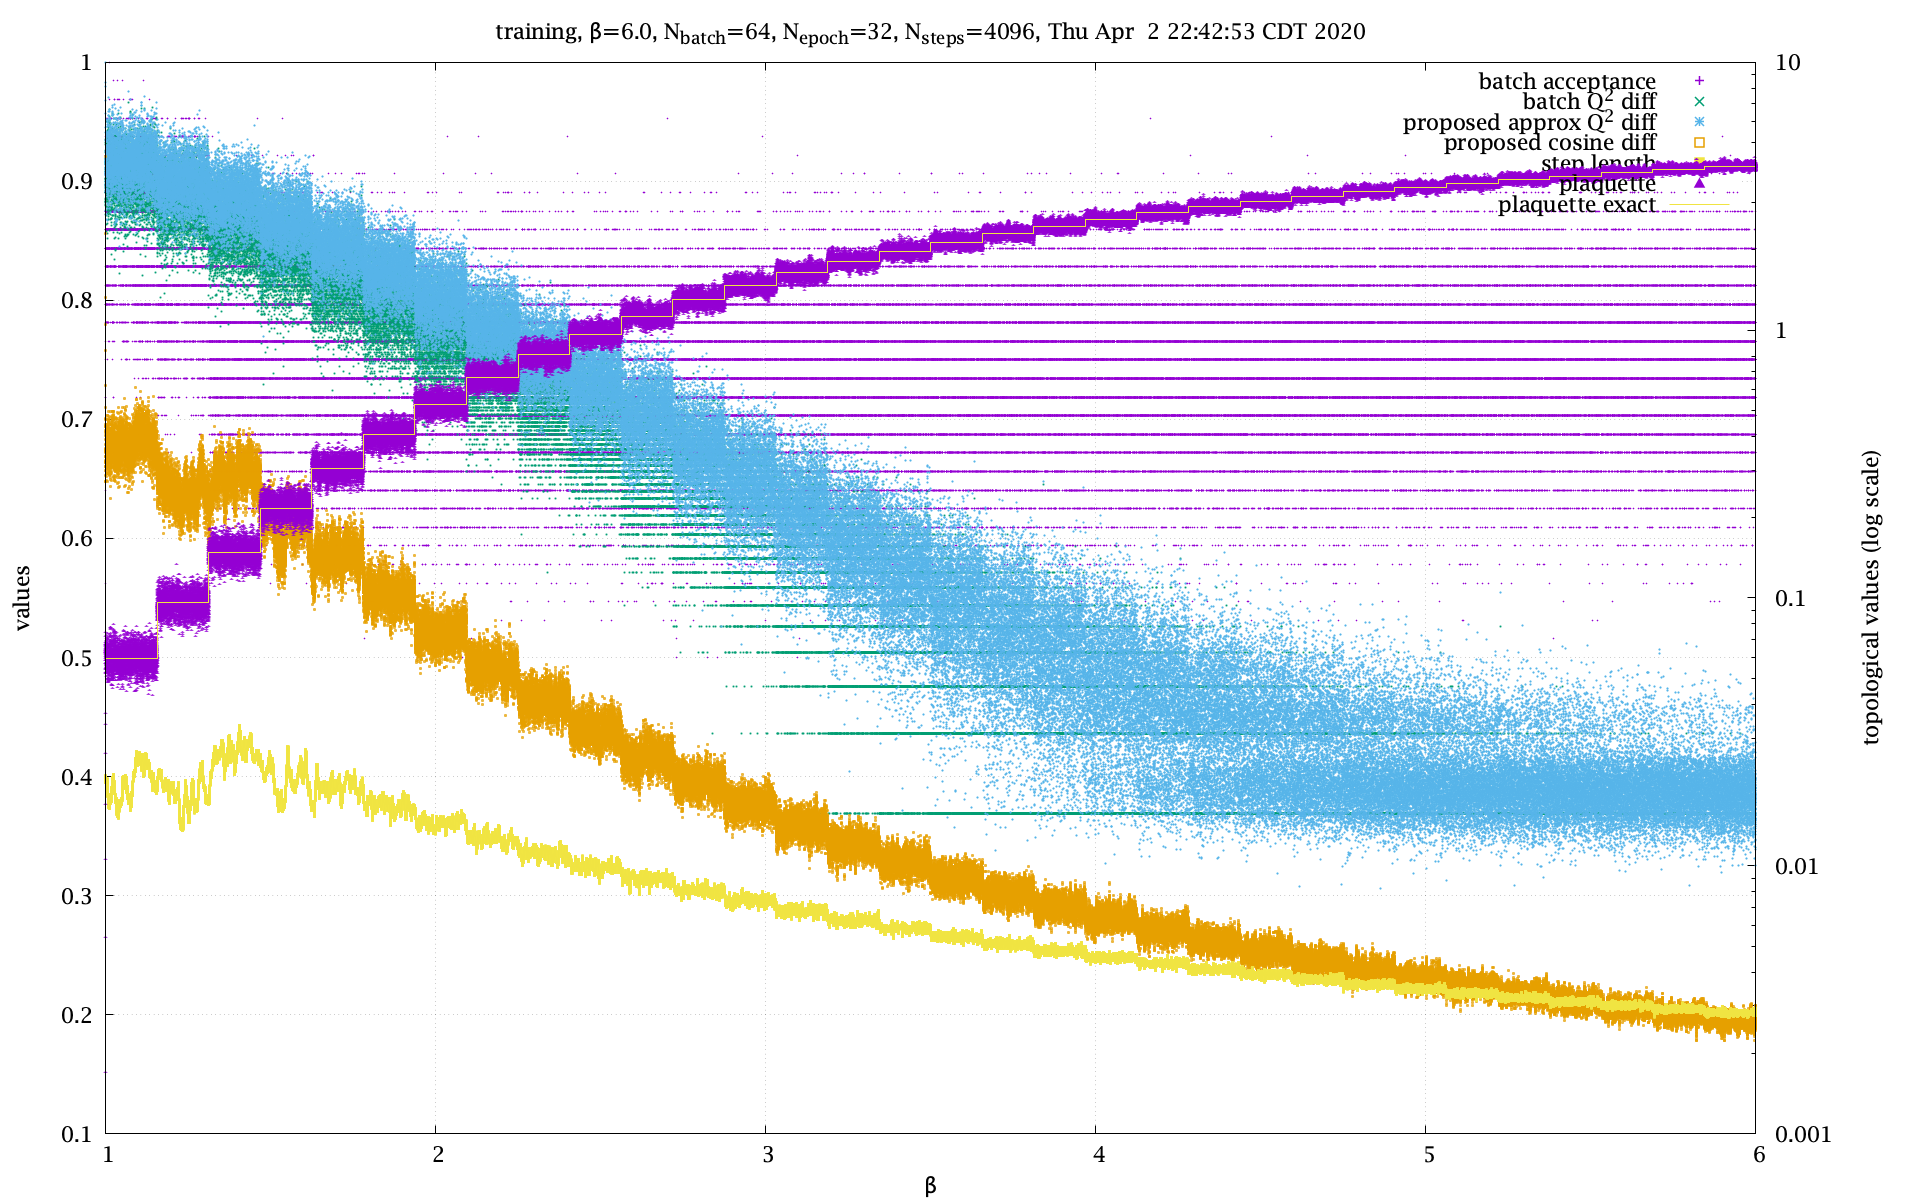
\includegraphics[width=\textwidth]{../../u1_2d/t4.png}
	\caption{\label{training-4}Annealed training steps for $V=8×8$ for HMC with 10 leapfrog steps,
	The only trainable parameter is the step size.}
\end{figure}

\begin{figure}
	\centering
	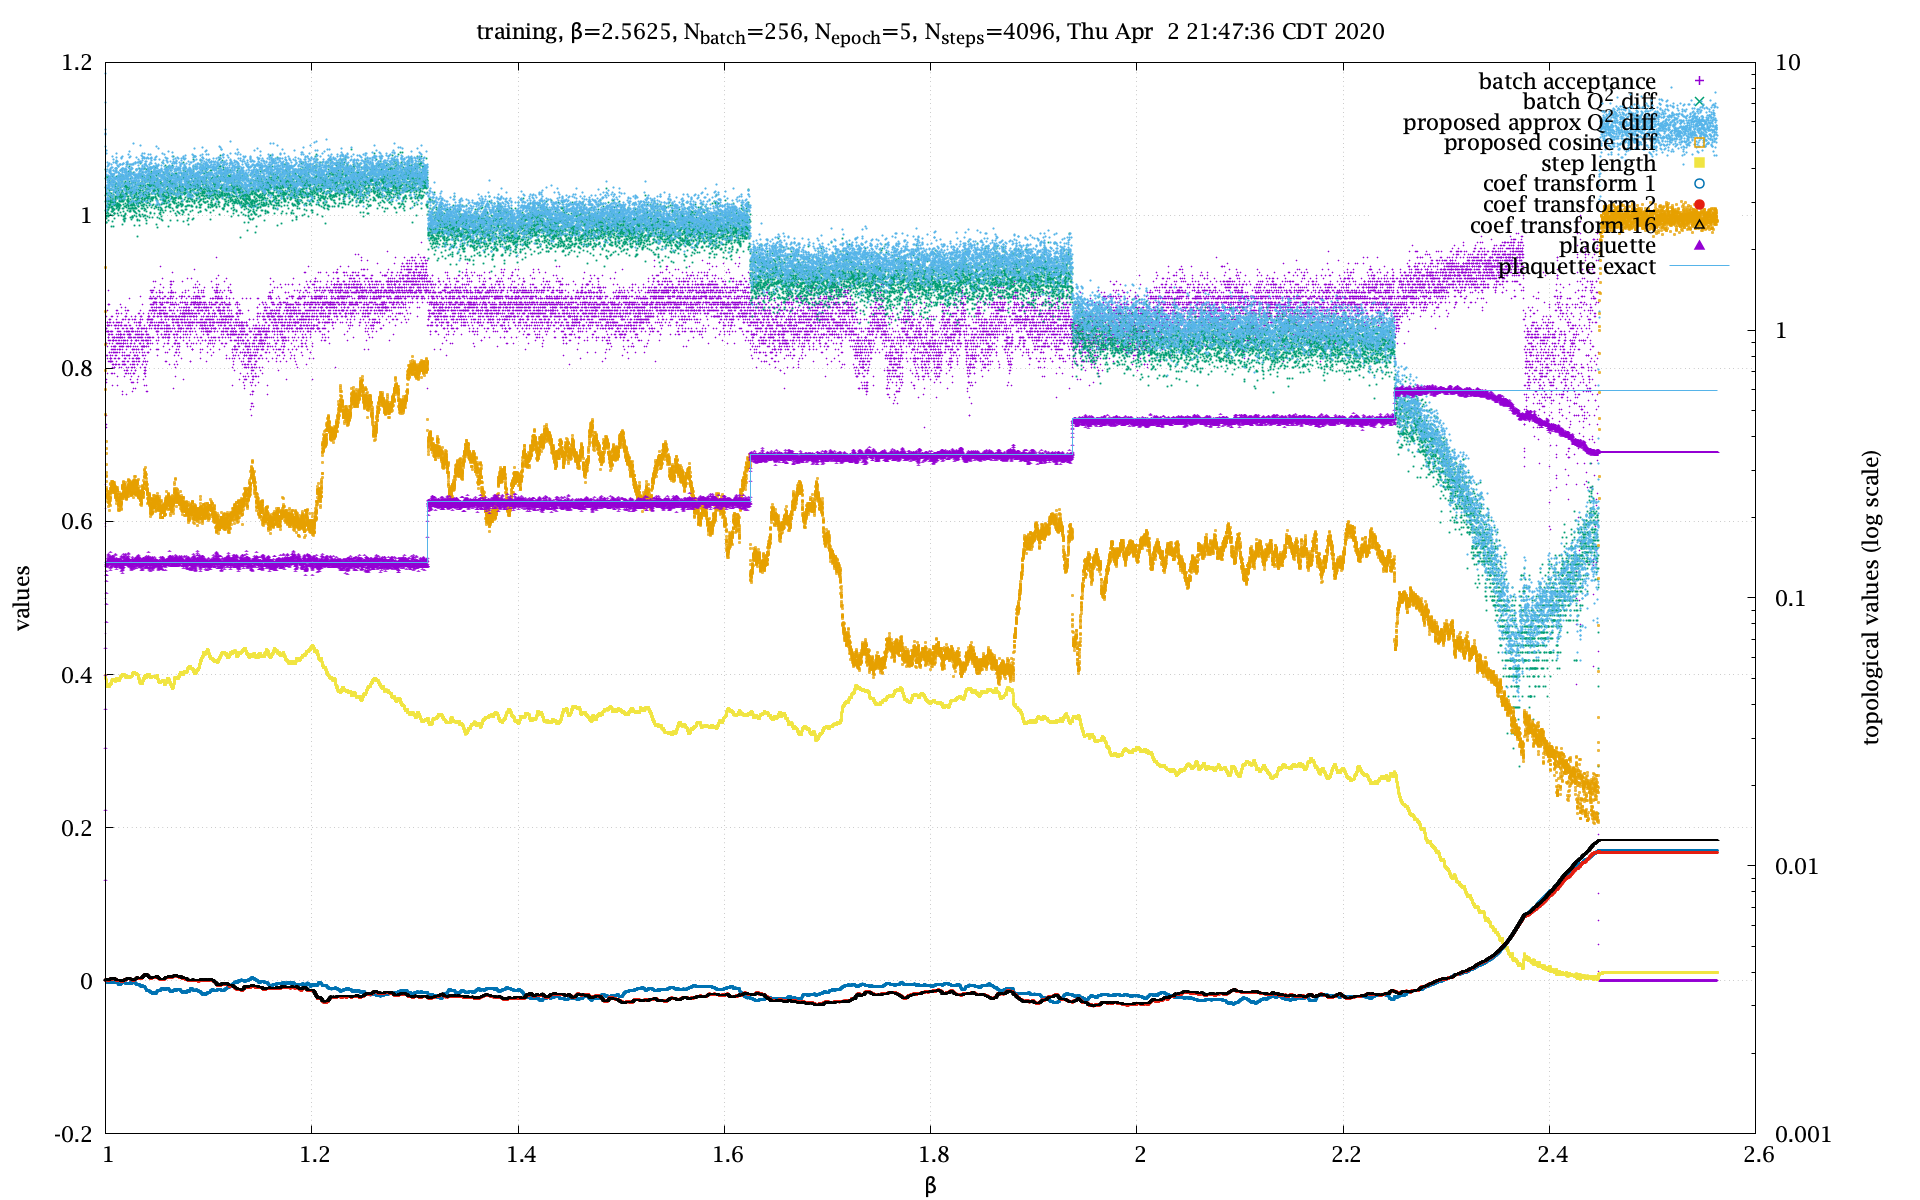
\includegraphics[width=\textwidth]{../../u1_2d/t2.png}
	\caption{\label{training-2}Annealed training steps for $V=8×8$ with 10 leapfrog steps.}
\end{figure}

\begin{figure}
	\centering
	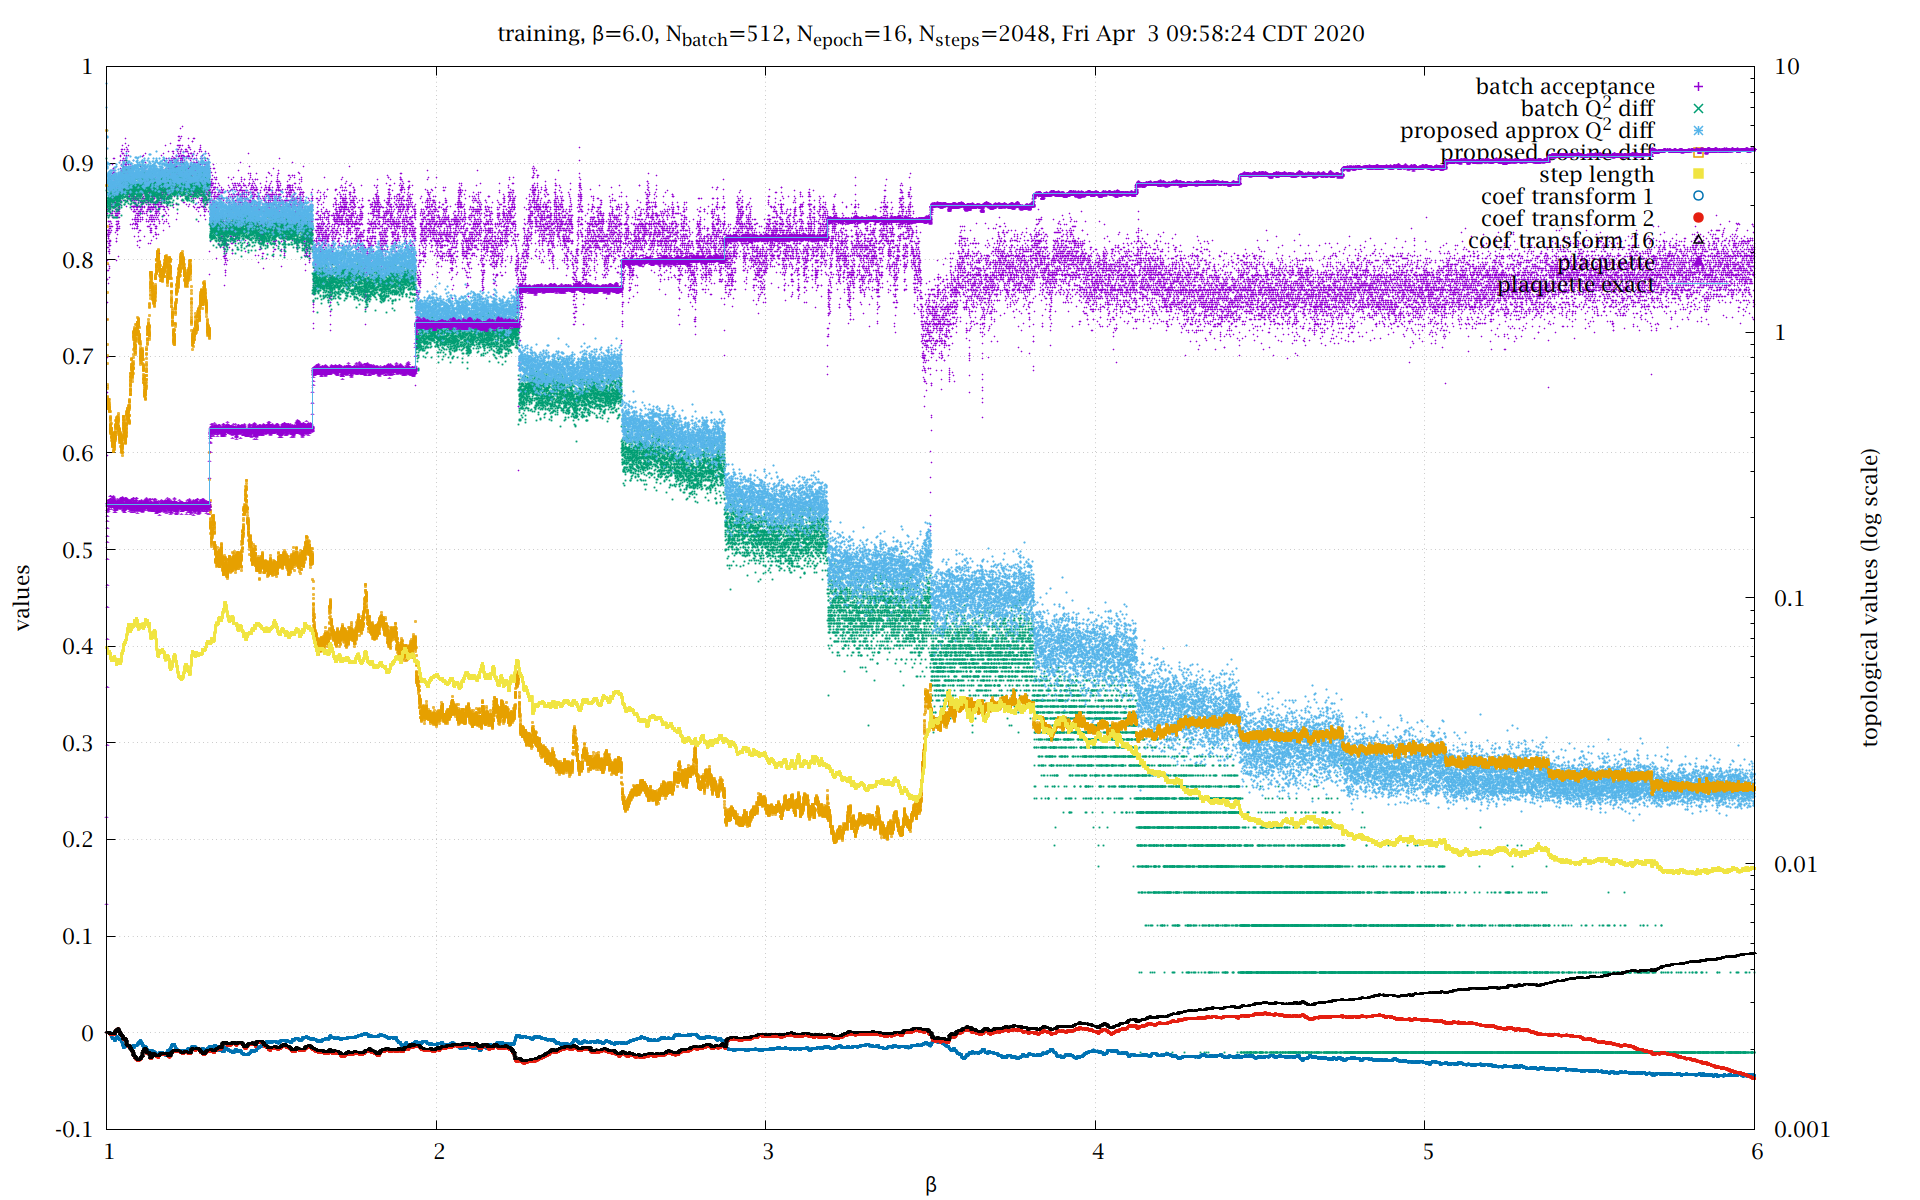
\includegraphics[width=\textwidth]{../../u1_2d/t5.png}
	\caption{\label{training-5}Annealed training steps for $V=8×8$ with 10 leapfrog steps.}
\end{figure}
